\documentclass[a4paper,12pt]{article}
\usepackage[slovene]{babel}
\usepackage[utf8]{inputenc}
\usepackage{multicol}
\usepackage{fullpage}
\usepackage{guitar}
\usepackage{titlesec}
\usepackage{graphicx}
\setcounter{secnumdepth}{-1} 
\usepackage[absolute]{textpos}
\titleformat{\chapter}{\large\bfseries}{\thesection}{1em}{}
\titleformat{\section}{\Large\bfseries}{\thesection}{1em}{}
\titleformat{\subsection}{\large\bfseries}{\thesection}{1em}{}

\begin{document}
\pagenumbering{Roman}
\begin{titlepage}
\begin{textblock*}{297mm}(-6mm,-0mm)
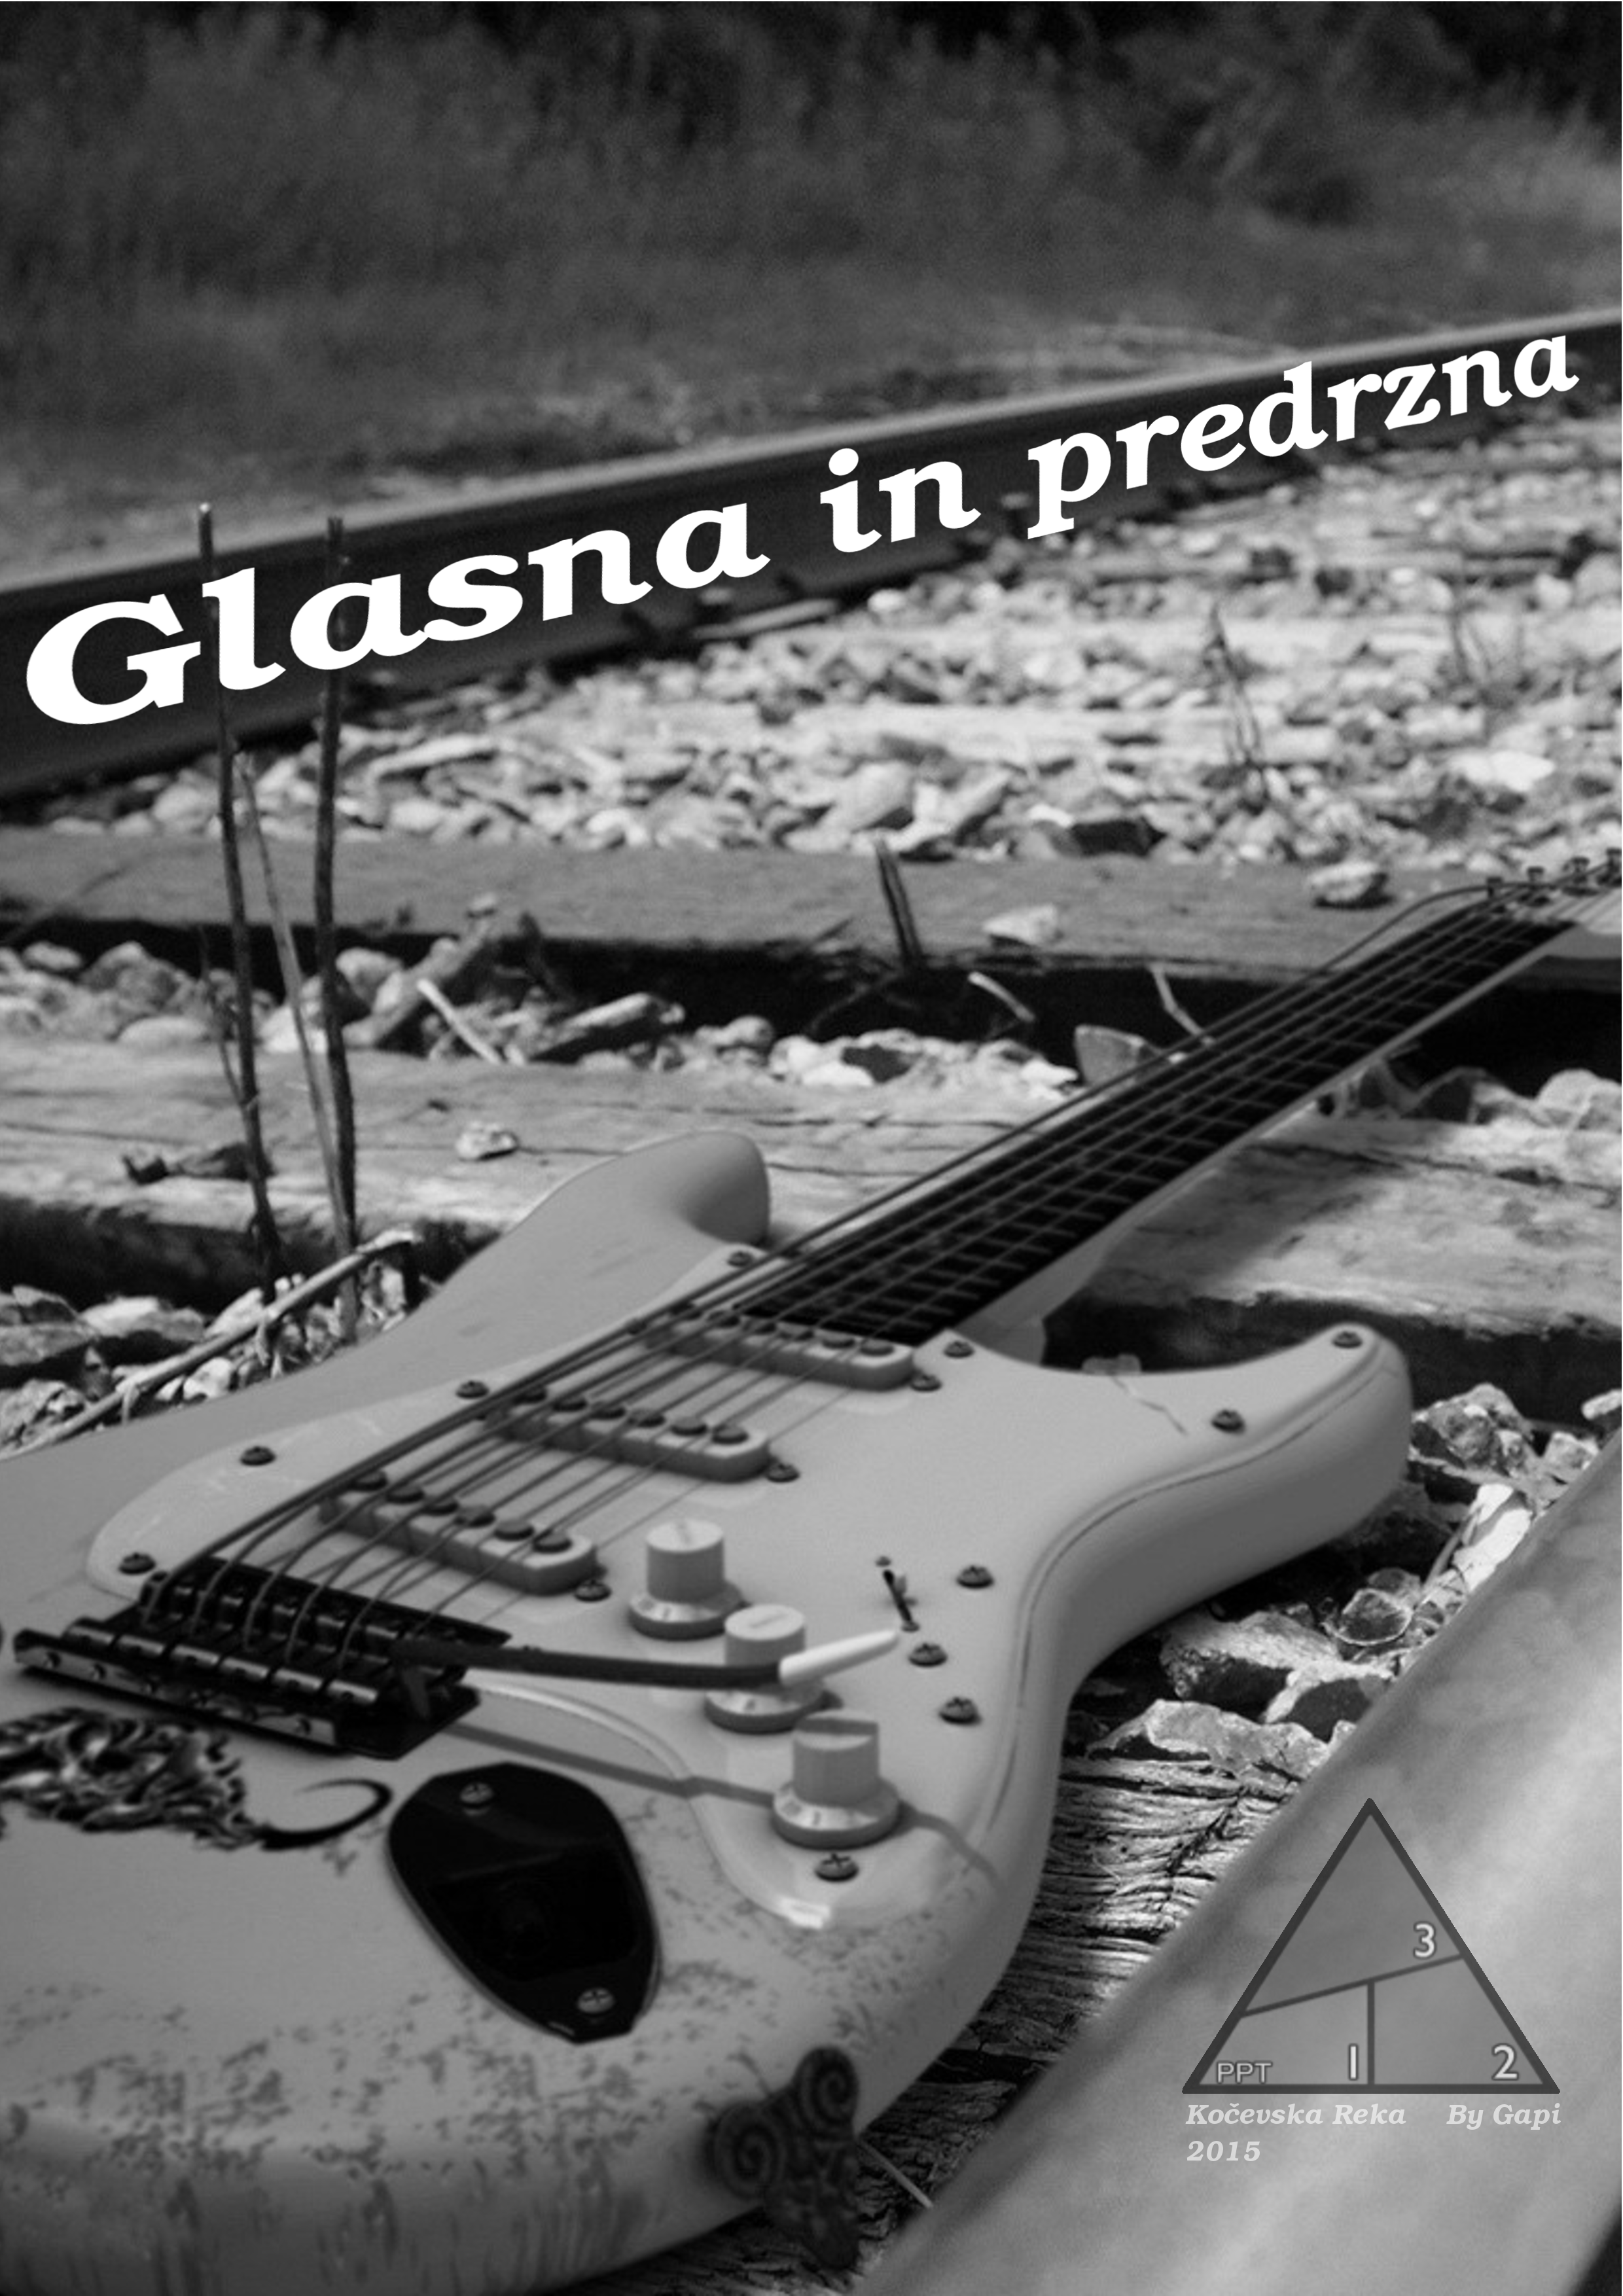
\includegraphics[width=\paperwidth]{img/tpage.png}
\end{textblock*} \
\end{titlepage}
\setlength{\columnseprule}{0.5pt}
\begin{multicols}{2}
\tableofcontents
\end{multicols}
\pagebreak

\setlength{\columnseprule}{0.5pt}
\begin{multicols}{2}
\pagenumbering{arabic}
\section{Akordi}
\begin{guitar}
[A - X02220  Am - X02210]

[B - X13331  Bm - X13321]

[C - X32010  Cm - X35543]  

[D - XX0232  Dm - XX0231] 

[E - 022100  Em - 022000] 

[F - 133211  Fm - 133111]

[G - 320003  Gm - 355333]

[H - X24442  Hm - X24432]


[A7 - X02020  B7 - X13131]

[C7 - X32310  D7 - XX0212]

[E7 - 020100  F7 - 131211]

[G7 - 320001  H7 - X21202]


[Am7 - X02010  Bm7 - X13121]

[Cm7 - X35343  Dm7 - XX0211]

[Em7 - 022030  Fm7 - 131111]

[Gm7 - 353333  Hm7 - X24232]


[C# - X46664  D# - 779997]

[F# - 244322  G# - 466544]


[C#m - X46654  D#m - 779987]

[F#m - 133111  G#m - 466444]


[A6 - X02222  C6 - X055555]

[D6 - X077777 E6 - X099999]


[ASUS2 - X02200]

[ASUS4 - X02230]

[DSUS2 - XX0320] 

[DSUS4 - XX0233]

[ESUS4 - 022200]

[CMAJ7 - X32000]

[FMAJ7 - 103210]

[GMAJ7 - 3X0032]

[DADD4/ADD2 - 554030]

\end{guitar}
\subsection*{Barre akordi}
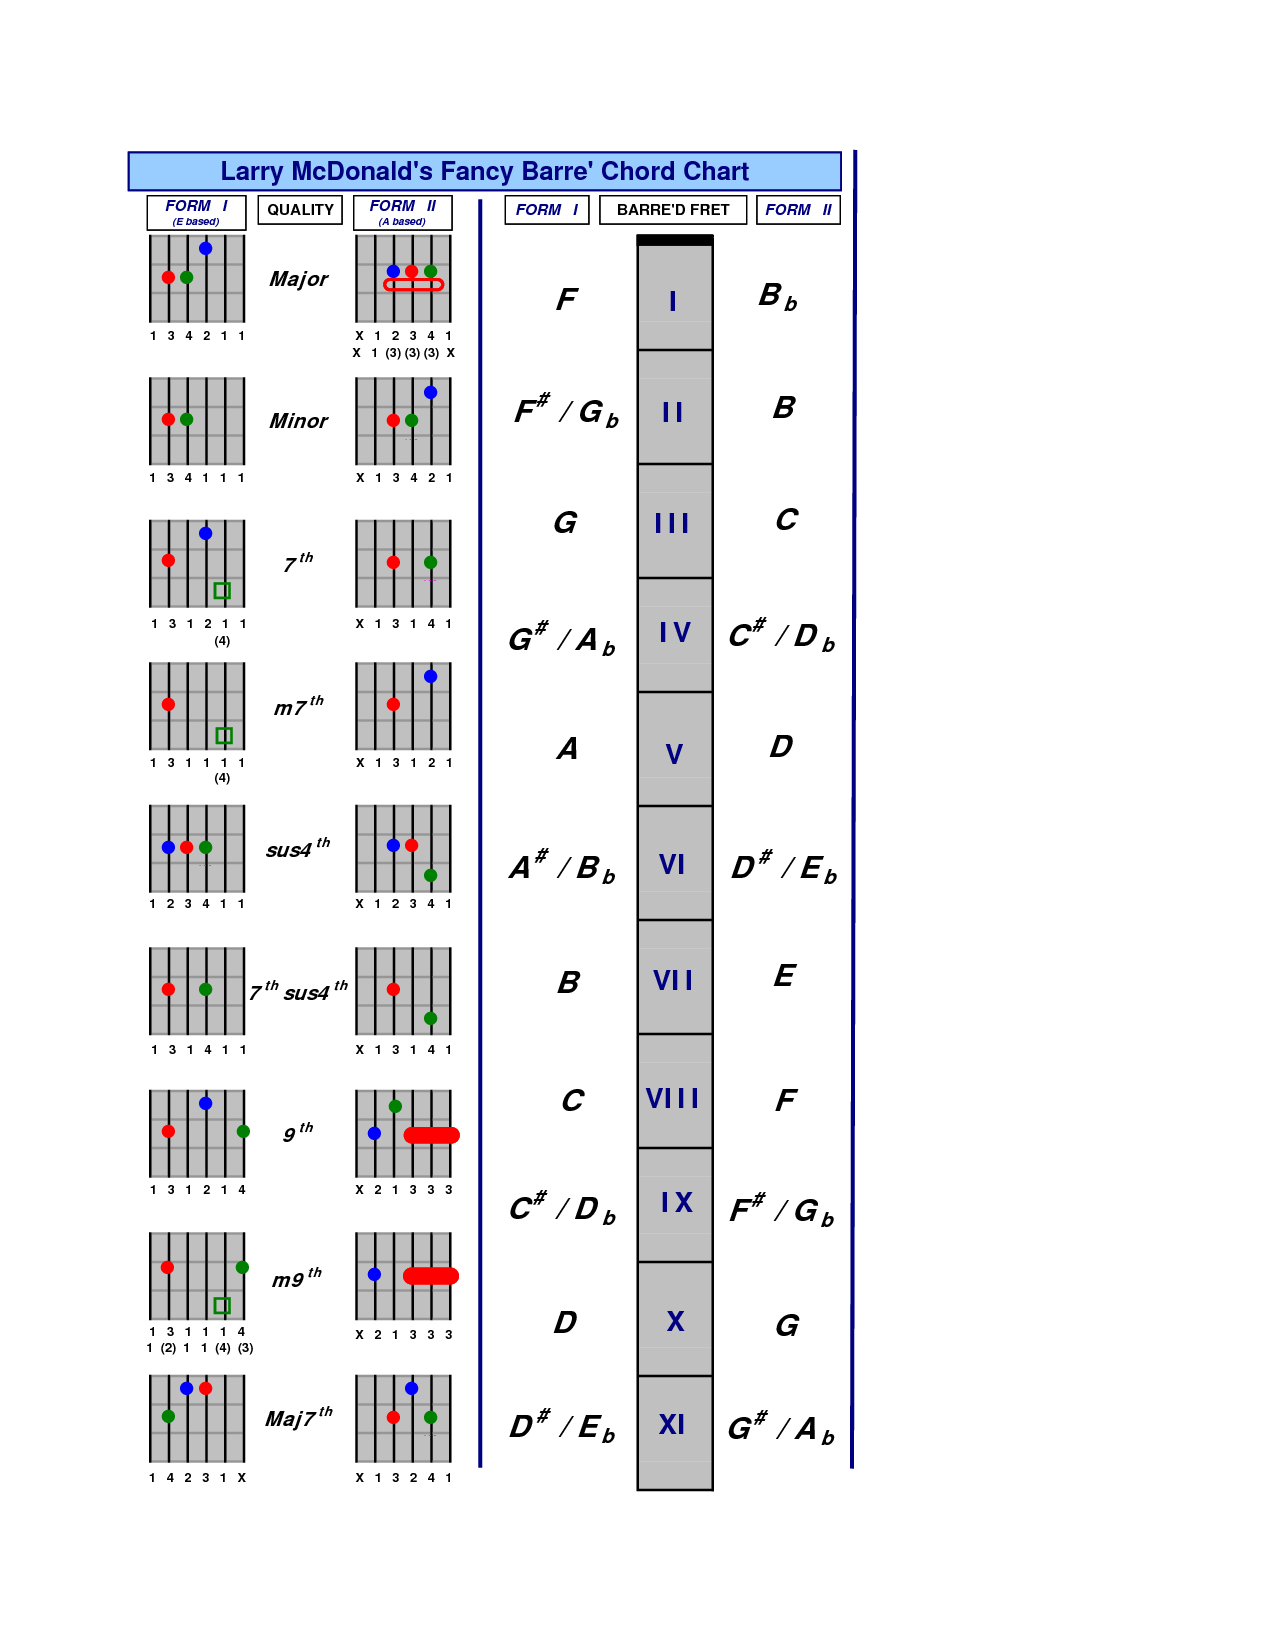
\includegraphics[width=140mm]{img/barre.png}
\clearpage
\section{442 do Beograda}
\subsection*{Bajaga}
\begin{guitar}
[F A# 	F  Gm Gm F 2x]

[F]Ja imam krvotok od bencina,
pred mojim [A#]očima ravan [F]put,
ovo je žestoka ma[Gm]sina,
nebo mastilo, mesec [F]zut.

Nisam blesav, da brojim zvezde,
brojim znake i linije,
psi laju na karavane,
a karavane prolaze.

Kao tanak snar šušti prašina,
442 do Beograda,
gume škripe blues kilometara,
442 do Beograda.

solo

mozak radi na kiseonik,
ljubav okreče točkove,
motor svetli ko svetionik,
brzina skida okove.

Nisam blesav...

Kao tanak snar...

solo

Ja imam krvotok od...

Nisam blesav...

Kao tanak snar... 
\end{guitar}
\section{Da te vidim golu}
\subsection*{Babe}
\begin{guitar}
Ako me [G]voliš, dokaži to [C]i ne uzimaj za zlo
Što sam brz [G]bio, [F]kratko te [C]ljubi[G]o.
U tvome oku ne vidim sjaj, slutim i na skori kraj.
Baš mi se ne da, djavo me ujeda.

	     
[G]Da te vidim golu  ( daj da te vidim golu ) 
[C]na severnom polu ( na severnom polu ) 
[G]Da te vidim golu, [F]to sam po[C]zele[G]o.

Ti si za mene svetinja, ustvari si avetinja.
Ne budi takva veštica opaka.
U noči punog meseca, strah mi dušu preseča.
Srce mi kalnu na tebe brutalnu.

Da te vidim golu ( daj da te vidim golu ) 
na severnom polu ( na severnom polu )
Da te vidim golu, to sam poželeo.

\end{guitar}
\section{Dobro jutro}
\subsection*{Bajaga}
\begin{guitar}
[D]Dobro [G]jutro, [D]ovo iznad [A]nas je nebo
[D]Zna da [G]bude [D]kad je sunčan [A]dan
[D]Svetlo [G]plavo, [D]bistro dubo[A]ko i vedro
[D]Suncu [G]staza [D]a zvezdama [A]stan


Dobrodošli ova pesma to su ptice
Zatrepere kad je mesec pun
Lete nebom i pevaju kada sviče
Perje, krila, kap, duše i kljun


Dobrodošli pozdravlja vas divlje cveče
Sladak miris ima svaki cvet
Strast i ljubav, zuje pčele opijene
To je ono što pokreče svet

\end{guitar}
\section{Đurđevdan}
\subsection*{Bijelo Dugme}
\begin{guitar}
[Am]Prole[G]ce na moje [C]rame sleće 
[Dm]Durđevak [Am]zeleni 
[Dm]Durđevak [Am]zeleni
[F]Svima [G]osim [Am]meni


Drumovi odoše, a ja ostah, 
nema zvijezde danice
Nema zvijezde danice, 
moje saputnice.


E i kome sada moja draga 
na đurđevak miriše
na đurđevak miriše, 
meni nikad više.


[C]Eee ee [Dm]eee 

[Am]Evo zore, [Dm]evo zore, [Am]bogu da se [Dm]pomolim 
[Am]Evo zore, [Dm]evo zore, [F]ej Đuđevdan je 
[Dm]A ja nisam [F]s onom [G]koju [Am]volim   


E i kome sada moja draga 
na djurdjevak miriše
na djurdjevak miriše, 
meni nikad više.


Njeno ime neka se spominje 
svakog drugog dana
Svakog drugog dana 
osim đurđevdana.

         
Eee-ee-eee...

\end{guitar}
\section{Gorska roža}
\subsection*{Andrej Šifrer}
\begin{guitar}
[D]Odšel bom tja kjer je daljši dan,
kjer se [G]mestni svet kon[D]ca.
[D]Kjer namesto asfaltnih cest
[A7]vodi le steza. [D]


Hiše razpršene so
kot jata plahih jerebic.
Čas utripa drugače če živiš
v eni od gorskih vasic.


Tisti večer sem žganje pil,
kot ga pije gospodar.
Bog mi v jezik je dal moči
in takrat sem jo spoznal.


Soseda mlada prisedla je
srečal njene sem oči.
Ko smo peli sem jo gledal,
kako se mi smeji. [D7]

  
[G]Gorska roža [D]caka me,
[A7]gorska roža, da [D]vrnem se,
[G]moji Špeli [D]iz planin,
[A7]pod srcem pustil [D]sem spomin.


Brez staršev je, a fantov ni,
ki bi ženili se v gore.
Zjutraj gre v tovarno
saj z majhno kmetijo pač ne gre.


Vzela me je čeprav sem bil
zanjo skoraj še otrok.
Naučila me je piti med,
a jaz sem dal ji svojih 18 let.


Gorska roža...


Od takrat sem pri njej živel,          
na gruntu ob koncu vasi.
Čez dan kitaro sem igral 
in ljubil Špelo vse noči.


Bil opran sem in vedno sit,
jedel kruh sem iz njene peči.
Vstajala je zgodaj, na delavski
avtobus se vedno mudi.


Gorska roža...


Ko zadnja košnja v kozolcu je,
čutiš hladen že objem.
Postajal sem nemiren, 
saj začutil sem jesen. 


Ki pravi:


O dreja poglej okrog,
zdaj postal si del planin.
O dreja jaz se bojim, 
da nekoč te ne izgubim.

\end{guitar}
\section{Hvala za vijolice}
\subsection*{Bilbi}
\begin{guitar}
[E]Ta tvoja žena mi je [Am]ze pri[E]jatelj' [Am]ca 
ne vem, če [E]ne bi ji kar [Am]vse po[E]veda[Am]la 
da skupaj [E]smirava od[Dm]kar tvoj [C]mali [G]Jan 
v [Dm]vrtcu [C]je vsak [G]dan. 


Ko prvič prišel si skoz’ vrata nasmejan, 
prevzel me je občutek – »vse lahko ti dam«, 
zdelo se mi je, da pač tak’ si strašno sam, 
da rabiš nežno dlan. 


[Am]Hvala  za  vijolice,
[Dm]torbe, čevlje, vrtnice,
[G]vse parfume, ogrlice.
Kaj pa [C]tvoje srce?
Kaj pa [E7]tvoje ime?  [Am Dm G C E7 ]


Hvala za počitnice 
in prekratke vikende, 
verze mal’ pocukrane. 
Kaj pa tvoje srce? 
Kaj pa tvoje ime? 


Postala sem čisto ta prava ljubica, 
kar dolgo časa nisem se zavedala, 
potem obljubljal si mi, da boš jo pustil, 
da boš se preselil. 


Ne upam ti pokazat, da mi je hudo, 
ker vse, kar primeš, ljubi, pade ti iz rok, 
ker zadnje čase nič več nisi nasmejan, 
z menoj si zadržan. 


Hvala za vijolice...

\end{guitar}
\section{I shot the sheriff}
\subsection*{Bob Marley}
\begin{guitar}
[Em]I shot the sheriff
[Am]But I [Bm]didn't shoot 
no [Em]deputy, oh no! Oh!
[Em]I shot the sheriff
[Em]But I [Bm]didn't shoot 
no [Em]deputy, ooh, ooh, oo-ooh.


[C]All a[Bm]round in my [Em]home town,
They're [C]tryin' to [Bm]track me [Em]down;
They [C]say they want to [Bm]bring me in [Em]guilty
For the [C]killing of a [Bm]depu[Em]ty,
For the [C]life of a [Bm]dep[Em]uty.


But I say:
I shot the sheriff
But I swear it was in self-defence. 
I say: I shot the sheriff - Oh, Lord! -
And they say it is a capital offence. Yeah!


Sheriff John Brown always hated me,
For what, I don't know:
 Every time I plant a seed, 
He said kill it be-fore it grow
He said kill them be-fore it grow 


And so:
I shot the sheriff
But I swear it was in self-defence.
I shot the sheriff
But I swear it was in self-defence. 


Freedom came my way one day
And I started out of town, yeah!
All of a sudden I saw sheriff John Brown
Aiming to shoot me down,
So I shot - I shot - I shot him down and I say:


I shot the sheriff
But I didn't shoot no deputy, oh no! Oh!
I shot the sheriff
But I didn't shoot no deputy, ooh, ooh, oo-ooh.)


Reflexes had got the better of me
And what is to be must be:
Every day the bucket a-go a well,
One day the bottom a-go drop out,
One day the bottom a-go drop out.


I - I - I - I shot the sheriff.
Lord, I didn't shot the deputy. Yeah!
I - I (shot the sheriff)
But I didn't shoot no deputy, yeah! No, yeah!

\end{guitar}
\section{Imagine}
\subsection*{Beatles}
\begin{guitar}
[C]Imagine there's no [F]heaven.
[C]It's easy if you [F]try.
[C]No hell be[F]low us.
[C]Above us only [F]sky.
[F]Imagine [Am]all the peo[D7]ple [G]living for today.
[G7]A-ha-aaa


Imagine there's no countries
It isn't hard to do.
Nothnig to kill or die for 
And no religion too.
Imagine all the people living  life in peace 
Yu-hu-uuu


[F]You may [G]say  i'm a [C]dreamer. [E E7]

[F]But i'm [G]not the only [C]one. [E  E7]

[F]I hope some[G]day you'll [C]join us [E  E]

[F]And the [G]world will [C]be as one.


Imagine no posessions.
I wonder if you can.
No needs for greed or hunger 
A brother hood of man.
Imagine all the people sharing all the world.
Yu-hu-uuu.


You may say  i'm a dreamer.
But i'm not the only one.
I hope someday you'll join us 
And the world will live as one.

\end{guitar}
\section{Inštruktorska balada}
\subsection*{Beatles}
\begin{guitar}
[C]Vso noč ko tabor spi, [C7]sanjarim o njej,
ki rada ima lepe [F]reči.
[Dm]To se [G]zgodi [C]vsakemu, ki [C7]ljubi.
Lah[F]ko se zgo[G]di vsake[C]mu.
 

Ko noč zagrne travo, tišina zažari,
me misel nate greje, saj vem, da blizu si.
Topot zadrg šotorov me plaši,
da nisi potegnila tudi ti.

 
Ne vleci dol zadrge šotora svojega,
noč, ki je pred nama, bo sreča za oba.
Vodstvo sestankuje, ostali so odšli,
jaz pa sam prepevam, prepevam [C7]si.	
 

Inštr[F]uktorka [G]moja in [C]jaz inštruktor [C7]tvoj
in [F]Gozdna šola [Dm]z nama, 
[G]zdaj gremo vsi v [G7]boj - ooooj.
 

Spomin na tiste dni, na zvezdnate noči
prikliče melodijo mladostnih nežnosti.
Glej jo čarovnijo, spet veter šelesti.
Spet mi v mislih pesem oživi.


Ne vleci dol...

\end{guitar}
\section{JA!}
\subsection*{B. Terpinc, M. Koren, M. Stergar, D. Novak}
\begin{guitar}
[C]Kako je lepa, [G]kako diši
[Am]Zjutraj v glavi se [F]mi zvrti
[C]Iz šotorov slišim [G]godrnjanje,
[Am]vsi podaljšali bi [F]svoje sanje.


[C]Na Kolpi je ful [G]dobr – [Am]JA
[C]Ce nisi tle ni [G]dobr – [Am]ja
[C]Plaža in ma[G]saža – [Am]JA
[C]U kuhni pa sta[G]laža - [Am]ja


Globoko v senci kjer sonca ni
nova misel se rodi.
Ti ob meni, utrip srca,
prisluhni gozdu in šumu voda.


Ref.


Tam ob ognju njene oči.
V srcu čutim da si me želi.
Ne, ne, ne, ne, ne bom več oprezen.
V akcijo da rodi se ljubezen.


Ref.

\end{guitar}
\section{Lepa janja}
\subsection*{Bajaga}
\begin{guitar}
[D]Maslina je oliva [A]mene sunce poliva
[Hm]procvale su kajsije [F#m]rumene
[G]pa se vidi jasnije
[D]pa se čuje glasnije
[A]na celom svetu od sto milja.


Mene sunce nervira
zrake loše servira
pa te dobro ne vidim ovaj put
onda vidim jebote 
nigde takve lepote
na celom svetu od sto milja.


[G]Ni[A]ko [Hm]lepsi nego [F#m]ti
[G]lepa Janja, [D]ribareva [A]kci.
Na celom [Hm]sve[F#m]tu le[Hm]pote takve [F#m]ni
[G]samo lepa [D]ribareva [A]kči.


Maslina je oliva mene sunce poliva
procvale su kajsije rumene
pa se vidi jasnije
pa se čuje glasnije
na celom svetu od sto milja.


Mene sunce nervira
Zrake loše servira
Istopi ti maskaru svaki put
Pa se ljutiš na mene
Pa mi tražiš zamene
Na celom svetu od sto milja.
      

Niko lepsi...


Onda pesme drugi deo
da promenim ja bih hteo
jer ne volim depresivne krajeve
zato želim ribarima puno sreče s vetrovima
i pune mreže ribe sveže.


Niko lepši nego ti
lepa Janja ribareva kči
na celom svetu lepote takve ni
samo lepa ribareva kči.
Na celom svetu niko kao ti
lepa Janja ribareva kči. 

\end{guitar}
\section{Lovro}
\subsection*{Big foot mama}
\begin{guitar}
[C Am Em G] 

[C]Caku je Lovro, [Am]caku vsak dan.
[Em]Caku je nevesto, [G]sovražu je bit sam.
[C]Zeleu si je vsaj enkrat ji [Am]modrček odpet,
[Em]saj mu brez nje tko [G]več ni blo za žvet.


In zvezde so sijale, gor na njen balkon,
a on je kr naenkrat zavrtu telefon.


[F]Rad bi biu s tabo [G]in bi se smeju spet,
[Am]ne da se mi več tok trpet,
[Am]ne da se mi več tok trpet.
[F]Rad bi biu s tabo [G]in bi se smeju spet,
[C]hočem te za sebe met,
[C]O hočem te za sebe met.

[C Am Em G] 

Že naslednjo noč ni preživu sam, 
predala sta se strasti,
nobenga ni blo sram.


A sreča ni bla dolga, pismo je pršlo,
bila je zaročena, nesla ga je okrog.


In nč mu ni blo jasn, 
le blo mu je hudo, 
za to noč bil je dobr, 
za več pa bl težko.


Rad bi bil s tabo...
 
[C Am Em G C Am]

Čaku je spet Lovro, čaku vsak dan.
Dočaku ni neveste, niti beli dan.
Napisu je le pismo in še njen naslov,
na vrtzu se je obesu, v smrt se je pognou. 

                         
[F]Ceprov bi rajš bil s tabo 
[G]in bi se smeju spet.
[C]Nism mogu več trpet,
O nism mogu več trpet.


Rajš bi bil s tabo... (2x)

\end{guitar}
\section{Mala terasa / Na vrhu nrbotičnika}
\subsection*{Bele Vrane}
\begin{guitar}
[C]Mala terasa in 
[F]spodaj Ljubljana, p[C]omanjšana,
da odnesla [G]bi od tu,
bele hiši[C]ce v predpasni[G]ku.

 
Tukaj s te male terase 
sredi Ljubljane ta hip lahko
bi dosegel Krim z roko.


Sva šla na [D#]malo teraso 
nad [G#]sirno Ljubljano,
da [D#]najina vsa Ljubljana [B]bi bila.


Na nebot[F#]ičnik sva odš[C#]la,
Bliže [D#m]sonca in modreg[G#]a neba, [C#]'
poza[F#]biva, da prem[C#]ajhna za dv[E]a 
in [H]zalostna [F#]sobic[G#]a je n[C#]ajina. [F#]'

\end{guitar}
\section{Ne u tojimi stili}
\subsection*{Ana Pupedan}
\begin{guitar}
[G]Ma ne, nej u tuojmi stili
Pustet me umret na konci bar[D]jače
[C]Ne nej u tuojmi [G]stili.


[G]Ma ženska mene u [D]postlo ma [C]greha [G]ne
[G]Lubezen v rakah [D]unga ku [C]neč ne [G]cuti
[G]Jest sm ti dal lu[D]bezen sm [C]mislu na [G]tebe
[G]In kaj si ti meni [D]dala?
[C]Vinu [G]grenku, [C]Vinu [G]grenku


[G]Ko sm prvič srečal jo je mela krive [D]noge
[D]Ko sm drugič srečal jo so [C]ble ko[G]smate
[G]Maaaa je primem za [D]vime
[D]Ko ga [C]porinem vse [G]mine


Ma ne, Nej U Tuojmi Stili
Pustet me umret na konci barjače
Ne Nej U Tuojmi Stili.


Ma ženska mene u postlo ma greha ne
Lubezen rakahunga ku neč ne čuti
Jest sm ti dal lubezen sm mislu na tebe
In kaj si ti meni dala
Škof vode.


[G]Za vogalom počepnite, eno kilo ga spus[D]tite
In u papir si ga zavite in domov si ga nesite
Da vam bo [D]lepo [C]smr[G]delo

\end{guitar}
\section{No woman no cry}
\subsection*{Bob Marley}
\begin{guitar}

[G  C  G  Am7  F  C  F  C  G]


[C]No [G]woman, no [Am]cry. [F]'
[C]No [F]woman, no [C]cry.  [G]'
[C]No [G]woman, no [Am]cry. [F]'
[C]No [F]woman, no [C]cry. [G]'


[G]Said, said,
[C]Said I re[G]member [Am]when we used to [F]sit
[C]In the govern[G]ment yard in [Am]Trenchtown.


[C]Oba, Ob[G]serving the [Am]hypocrites [F]'
[C]As they would [G]mingle
with the good people [Am]we meet, [F]'


[C]Good friends we [G]had oh 
[Am]good friends we've [F]lost
[C]al[G]ong the [Am]way. [F]'


[C]In this bright [G]future 
you [Am]can't forget your [F]past
[C]So dry your [G]tears I [Am]say And [F]'
  

[C]Ev'ry thing's gonna [G]be alright. 
[Am]Ev'ry thing's gonna [Fm]be al[G]right.
[C]Ev'ry thing's gonna [G]be alright.  
[Am]Ev'ry thing's gonna [Fm]be al[G]right.
[Am]Ev'ry thing's gonna [F]be alright 


No, [C]woman, no cry. [G  Am  F]'
No, no [C]woman, no [F]woman, no [C]cry. [G]'
[C]Oh, my little si[G]ster don't [Am]shed no [F]tears.
[C]No wo[F]man no cr[C]y. [G]


[C   G   Am   F   C   F   C   G]


[C]No [G]woman, no [Am]cry. [F]'
[C]No [F]woman, no [C]cry. [G]'
[C]Oh, my little [G]darlin', 
I say don't [Am]shed no [F]tears.


[C]No wo[F]man, no cr[C]y. [G]'
[C]Yeah little [G]darlin', 
don't [Am]shed no [F]tears.
[C]No [F]woman, no [C]cry. [G]'


And then Georgie would make a fire light
As it was log wood burnin' through the night.
Then we  would cook corn meal porridge
of which I'll share with you.


My feet is my only carriage,
So, I've got to push on through, 
but while I'm gone I mean...

\end{guitar}
\section{Prisluhni školjki}
\subsection*{Black and white}
\begin{guitar}

[F]Poletni [C]dan, ki je [B]mogoče že min[F]il 
in [B]mogoče šele [F]pride, poletni [C]dan. 


Poletni dan, ki ga morda nikdar ne bo 
in morda prišel ne bo od sonca zlat. 


Poletni dan, ki v školjko je ujet, 
ki ujet je v srce, vanj zakopan. 


Prisluhni šk[Dm]oljki, [B]

vanjo uj[Dm]et je, [B]
           
prisluhni š[Dm]koljki, 
          
[B]v njej po[C]letje ti šumi. 


Na uho te vabi, 
prisluhni vanjo, 
kako igra ti, 
vabi te za sanjami. 


Poletni dan, ki v školjko je ujet, 
ki ujet je v srce, poletni dan. 


Prisluhni školjki, 
vanjo ujet je, 
prisluhni školjki, 
v njej poletje ti šumi. 


Na uho te vabi, 
prisluhni vanjo, 
kako igra ti, 
vabi te za sanjami. 


Prisluhni školjki... 


Na uho te vabi... 


Prisluhni školjki... 

\end{guitar}
\section{Redemption song}
\subsection*{Bob Marley}
\begin{guitar}

Old [G]Pirates, yes, they rob [Em7]I.
Sold [C]I to the [G/B]merchant ships [Am]

[G]minutes after they took [Em]I 
[C]from the [G/B]bottomless [Am]pit.


But my [G]hand was made [Em7]strong
[C]By the hand [G/B]of the Almigh[Am]ty.
We fo[G]rward in this gener[Em]ation [C]triumphant[D]ly.


Won't you help to sing[G]   \

[C]thes[D]e songs of [G]freedom?
'Cause [C]all I [D]ever had[Em],    

[C]red[D]emption [G]songs,
[C]red[D]emption [G]songs. [C]
   
   
Emancipate yourselves from mental slavery,
None but ourselves can free our minds.
Have no fear for atomic energy,
'Cause none of them can stop the time.


How long shall they kill our prophets
While we stand aside and look?
Yes, some say it's just a part of it.
We've got to fulfill the book.

Won't you help to sing...

Emancipate yourselves from mental slavery,
None but ourselves can free our minds.
Have no fear for atomic energy,
'Cause none of them can stop the time.


How long shall they kill our prophets
While we stand aside and look?
Yes, some say it's just a part of it.
We've got to fulfill the book.


Won't you help to sing 
these songs of freedom?
'Cause all I ever had, redemption songs,
These songs of freedom, songs of freedom.



\end{guitar}
\section{Resničen svet}
\subsection*{Ana Pupedan}
\begin{guitar}
[G]Raje kot gledam te [D]crne oblake
[C]Raje odpravim se v [G]raj na sprehod.
[G]Kupim si liter [D]pravega žganja
In od[C]pravim se v predmestje ne[D]bes.


Opazujem ljudi poznane in tuje,
Ki zavračajo mi moj pogled.
Vzpostavljam tud stke z tistim početjem
Ki mi prej ni bilo všeč.


Panično iščem zavetje rešitev.
Rad našel bi kritje pred nevarnostjo.
Pulim lase si mencam si oči
Nekdo me gleda z radovednost.


Potujem od ene žrtve do druge
Pozorno pošlušam tegobe ljudi
Rad reši bi sebe rešil bi druge
A sploh ne vem če sm živ.


[G]Je to resničen svet ali [A]sanje 
ki jih preveč [D]dobro poznam?


Je to [G]sila peklenskega [A]zla 
ki odpira mi [D]vrata vsa?


Je to spo[G]min iz prejšnjega dela 
živ[A]ljenje ga [D]več ne pozna?


[C]Ali je to le živ[G]ljenje pijanca 
ki ga [D]noče nihče več poznat?


[C]Ali je to le živ[G]ljenje pijanca 
ki ga [D]noče nihče več poznat?


Počasi me spet žganje popušča
počasi se glava bistri
Počasi me spet strah spreletava
saj me kruta resničnost lovi.


Počasi spet vidim na pol manj ljudi
Kot sem videl jih užgan
Vidim tud nekaj ljudi s steklenico
Prazno pa žganju diši


Gledam te črne oblake na nebu
Še bolj so zdaj črni vsi.
Rad videl bi ptico na nebu
Ki ojlčno vejico v krempljih drži


Rad bi tudi da bi sonce me grelo
A tudi sonce zdaj več ne živi
Nimam denarja za še en liter žganja
In to me tudi najbolj skrbi


Je to resničen svet...

\end{guitar}
\section{Romanje}
\subsection*{Andrej Šifrer}
\begin{guitar}

[G]To je mesto, [Hm/F#]ki ne mara tujc[Em]ev
na c[G]estah s[Hm/F#]koraj da ni več ljudi.[Em]

Le f[C]antje s komun[Hm]ale so še b[Am7]udni
s ceste spr[H]ali bodo d[C]an in smet[G]i.
 

Ob desetih so zaprli vse lokale
v mestu je zavladal nočni mir.
Na železniško postajo se odpravim
tam edini točijo še nočni pir.


[G]Kot da tukaj m[Hm/F#]esto še ne sp[Em]i,
k[C]ot da tukaj m[Hm]esto še ž[Am7]ivi
romajo vs[C]i v barkah življenja
nosi jih v[D]eter alkoholnega vrenja
glej noč nam prin[C]aša novega gosta
nekaj boš sp[D]il in z nami odšel
na r[G]oo[Hm/F#]ooooooooooomanj[C]eeeee[D]eee,
r[Em]oooooo[D]oooooooomanj[C]e, [Am F#]

[Hm]na r[Em]ooooo[D]oooooomanj[C]e,
r[Am]oooooooooma[D]aaaaanj[Em]e.


Obraz izdaja, če noči so predolge,
roke izdajo, če težak bil je dan.
V oči upi pa govorijo drugo zgodbo
o vlaku, ki ga čakamo zaman.



\end{guitar}
\section{Ruski voz}
\subsection*{Bajaga}
\begin{guitar}
[Am  Fmaj7]

           
[Am]Voz, pospani [Fmaj7]voz za Harkov
[Am]Gomelj, Lenjin[Fmaj7]grad
[Am]Znam kako je [Fmaj7]nočas dalek [Am]

Beo[Fmaj7]grad



Neče [C]moči nika[G]da olov[Am]ka i harti[E]ja
i svi [C]ruski pošta[G]ri ne mo[Am]gu ti odne[E]ti
pismo [F]koje pišem [C]ja marka s [F]likom Lenji[C]na
i u [F]pismu jedi[C]na tuga [F]to me razbi[Am]ja.


Nije vodka rakija mada nocas udara
tuga mi je velika velika k'o Rusija
ja ne mogu poslati ljubav jer se ne salje
nit sam mogo poneti sobom tvoje poljupce.


Voz, u vozu izguzvana lica putnika.
Ti si tamo negde iza onih planina.


Da l' si mozda zaspala
Il' si budna kao ja
Da l' te muce nemiri
Il' te nista ne muci


Kada budes citala pismo koje pisem ja.
Tajna bice skrivena iza ovih redova.


Nije vodka rakija...

\end{guitar}
\section{Si še jezna name}
\subsection*{Bazar}
\begin{guitar}
[C]Si še jezna [C]name, 
saj sem čisto [Em]vse pozabil,
in bi rad te [F]spet povabil, 
če imaš kaj [G]casa zame.
Si še jezna [C]name, zdaj, 
ko je po[Em]letje mimo,
spomni se na [F]dolgo zimo, 
kdo te bo ob[G]jel čez rame?



[C]Ljudje govorijo, [Am]pamet delijo, pusti [Em]me, 
[C]lahko mi verjameš, [Am]ko me objameš, [Em]glej,
zunaj se [F]listje nabira, zunaj po [Am]snegu diši, 
burja že [F]polkna zapira, tebe pa [G]ni. 



Si še jezna name, 
zate sem doma pospravil,
jaz sem ti že šal pripravil, 
zdaj lahko zaupaš vame. 
Si še jezna name, 
jaz se ne bojim te zime,
veš, da mene zlahka prime, 
mnoge so še zmeraj same. 



Ljudje govorijo...

\end{guitar}
\section{Srečen z njo}
\subsection*{Botri}
\begin{guitar}
[D A]

[A]Kako pozab[D]im naj na zvez[A]dne  noci, [D]

[A]Kdo pogasi[Hm]l bo v meni og[F#m]enj  ki  tli, [Hm]

[F#m]Morda ne v[C]eš kako lahko bol[G]i,
Sedaj ko [A]tebe vec ni. [D A D]


Se ustavil mi bo cas kot takrat,
Bom lahko odkril še komu zaklad,
Bom še ljubil jo lahko tako,
Kot sem tebe samo.


Ko gledam jo, v nj[Hm]enih s[G]i oč[D]eh,
Še vedno cutim, v [Hm]njenih t[G]e  dlan[D]eh,
Bila si mi v[Hm]se, a pr[G]osim, p[D]usti  m[G]e, [Em]

Rad bi sr[A]ecen bil z njo[D]. [A D]

     
Kako pozabim naj vsa jutra besed,
In kdo zabrisal mi vecerov bo sled,
Lahko zaupam se še komu tako,
Da tega žal mi ne bo.


Kako pozabim naj na zvezdne noci,
Kdo pogasil bo v meni ogenj, ki tli,
Morda ne veš, kako lahko boli,
Sedaj ko tebe vec ni.


Ko gledam jo...

                
Ko gledam jo, v njenih si očeh,
Še vedno čutim, v njenih te dlaneh,
Bila si mi vse, a prosim, pusti me,
Rad bi s[A]rečen bil z nj[C]ooo     ...  o[G]oo, 
rad bi srecen bil z nj[D]o.
u[C]uuuuuuu ... uu[G]uuuuuuuu ... u[D]uuuuu ...


[Em  G  A]           

Kako pozabim naj na zvezdne noci,
Kdo pogasil mi bo ogenj, ki tli,
Morda ne veš, kako lahko boli,
Sedaj ko tebe vec ni.


Ko gledam jo... (2x)


Ko gledam jo, v njenih si oceh,
Še vedno cutim, v njenih te dlaneh,
Bila si mi vse, a prosim, pusti me,
Rad bi s[A]recen bil z nj[C]ooo  ...  o[G]oo, 
rad bi srecen bil z nj[D]o.


\end{guitar}
\section{Tamara}
\subsection*{Boris Novković}
\begin{guitar}

[E]očas sam ti opet [Am]sam, 
[F]da me barem nešto udar[G]i. [E]

Bit če rata kažu s[Am]vi, 
[F]a ja ču umrijeti od [G]ljubavi.[E] 



Ko mi tebe [F]uze, [G]Tamar[C]a, 
prodala si [F]suze [G]drugi[C]ma, 
nočima ja [F]sanjam tvoje [G]trago[C]ve, 
kuda idu [F]izgubljene [G]dje[E]voj[Am]ke. 

\end{guitar}
\section{Tamara}
\subsection*{Bajaga}
\begin{guitar}

Ispred teat[C]ra Baljš[G]oj,
ja sam te [Am]cekao [F]satima.
Tvoj beli [C]hrt Ber[G]zoj 
je [Am]lajao pred [F]vratima.


Na minus dvadeset i šest,
Moskva je tonula u san.
Ja sam se topio k'o sneg 
kada ga staviš na dlan.[F G]


[Am]Tamara,
[G]cekanje me strašno [Am]zamara,
[G]bele noči vetar [Am]samara,
[G]a tebe ne[F]ma.


Tamara,
nikad nije bilo tužnije,
da smo samo malo južnije,
negde dole južno.


A ja sam bio strešno kul 
i nisam padao na fore,
da li je tako bilo hladno 
i mornarima sa Aurore? 
Mada si bila lepša od Neve
i raskošnija od jermitaža 
ne bi te ček'o ni Žilber Beko,
to bi za njega bila blamaža.

\end{guitar}
\section{Tišina}
\subsection*{Bajaga}
\begin{guitar}
[Am]Mrak se skupio u [C]kap
Rano jutro kao [G]slap
Ulazi u sobu  [Am]


Dal' si ikad pitala
Tamne senke zidova
Ujutro gdje odu


Oci su ti sklopljene
Usne su ti umorne
Ne ljubi me njima


Nisu cvorci pjevali
Dok' je iznad krovova
Svirala tisina


Hajde Boze budi drug
Pa okreni jedan krug
Unazad planetu


Noc je kratko trajala
A nama je trebala
Najduza na svijetu


U mom oku samo hlad
U mom srcu samo stud
Inje i prasina


Nisu cvorci pevali
Dok je iznad krovova
Svirala tisina


Slusaj, gore pisti voz
Njime odlazim u Oz
Necu da se vratim


Sto god tebi napisem
Pocepam i obrisem
Al' ti moras znati


Nisi se probudela
Zato nisi videla
Igrale su sene


Nek' te dobri drugovi
i kraljevski orlovi
cuvaju od mene.

\end{guitar}
\section{Uspavanka za Evo}
\subsection*{Andrej Šifrer}
\begin{guitar}

Vsaka [G]zvezda na [Em]nebu [Am]zami[D]zi, 
teta [G]Luna pri[Em]kima, [Am]se zasme[D]ji. 
Poga[G]sili [Am]smo v[Hm]se luči, 
da naša [C]Eva lah[D]ko zas[G]pi. 


Vsaka zvezda na nebu zamiži, 
teta Luna prikima, se zasmeji. 
Pogasili smo vse luči, 
da naša Eva lahko zaspi. 


Pa naj z[Em]aspi, naj skrije svoje [D]trudne oči, 
pa naj za[Em]spi, da se malo sr[D]ce umiri 
in naj [G]sanja le o [Am]lepih stvareh. 
Ko [C]sonce zbudi jo, na ustih bo [D]smeh. 


Vsaka zvezda na nebu zamiži, 
Evin kužek zalaja, se poslovi. 
V kraljestvo škratov, sanj in vil 
jo nese sila nevidnih  kril. 


In že leti daleč proč od tega sveta, 
od tega kar ne razume in kar ne pozna, 
saj jo čaka svet drugačen od sanj. 
Kako naj svarim jo, kaj rečem ji v bran? 


[C]Boj se ljudi, ki ne [Am]znajo jokati, 
ne [G]gledajo v oči in ne [D]znajo stisnit’ dlan! 
[C]Boj se množic, ki [Am]mahajo s pestmi, 
šo[G]ferjev s klobuki, [D]nabitih na volan! 


Pa naj zaspi... 


Vsaka zvezda...

\end{guitar}
\section{Vsaka rwža jma trn}
\subsection*{Ana Pupedan}
\begin{guitar}
[C]Uba sva bla sred Paljške gmajne, 
ku se [F]j dejlou dan
[C]Bla sva taku ukep, da [F]blo ni za vrjet
[C]Uuu [F]Uuu, ka[C]ku mraz je [F]blu
[G]Aaaaa, če se [F]spunm me še zdej randa


[C]Vsaka rwža jma [F]trn
[C]Vsaka nouč jma [F]jutru
[C]Vsak kau[G]bojc puje [Am]eno in [F]isto
[C]Vsaka rwža jma [F]trn


Poslušam radio 94, na katermi je resničen svet
DJ Krmpi se zavrti, vsak večjer u Tangoti
Uu Uu, na mwurš taku
Aaaaa, kašna bala


Vsaka rwža jma trn...


Nikul n bom pozabu dnjeva, 
ku smi przadjela hudo bolečino,
Kr ljudje smo u čevljeh 
in ti smi s pjeto stwupla na pauc


Uba sva bla sred Jurške gmajne, 
ku se j dejlou dan
Bla sva taku ukep, da tu nej za verjet
Uu Uu, kaku mraz je blu
Aaaaa, če se spunm me še zdej randa


Vsaka rwža jma trn...

\end{guitar}
\end{multicols}
\clearpage
\clearpage
\null
\vfill
\center

\includegraphics[width=100px]{img/licence.png}

Pesmarica je zaščitena z licenco CC-BY-NC-SA. Vse pesmi so delo in last avtorjev. Morebitne napake in predloge sporočite na pesmarica.info@gmail.com 

Izvorna koda (LaTeX) ter PDF sta dostopna na https://github.com/gztproject/Pesmarica
\end{document}
